\documentclass[10pt]{article}
\usepackage{icmlko}

\icmlmeta{IP 파운데이션 월드모델}{203}{혼자 할 수 있는지는 알겠는데 함께 할지는 모르겠다}{모바일이 세 노트 연속 풀에서 빠져야 하는 유일한 도메인이었다. 조건을 찾았고, 찾고 보니 그것으로는 배치를 못 정한다}

\begin{document}

\twocolumn[
\icmlheader

\begin{abstract}
노트 197 · 201 · 202 에서 모바일만 세 번 연속 ``풀에서 빼야 하는 도메인''이었고
혼자 학습한 $\rho$ 가 $+$0.514 로 제일 높다. 노트 202가 ``그 조건을 알면 새
도메인을 자료 보기 전에 배치할 수 있다''로 닫았다. 후보 일곱을 쟀다 --- 학습 ·
유보 표본 크기 · 축 덮음 · 축$\leftrightarrow$라벨 상관(평균 · 최대) · 시간
안정성 · 라벨 묶임. 도메인 일곱으로 재면 축상관최대($+$0.61)와 덮음($-$0.61)이
공동 1위인데, \textbf{하나씩 빼 보니 셋이 부호가 흔들린다} --- 특히 학습 표본
크기는 웹툰 하나를 빼면 $-$0.03 에서 $+$0.77 로 뒤집힌다. 점을 늘렸다 ---
도메인을 반으로 쪼개 조각 열둘로. \textbf{셋만 살아남는다}: 덮음
\textbf{$-$0.60} · 마스크 변이 \textbf{$+$0.57} · 시간 변화 \textbf{$-$0.50}.
\textbf{축상관최대는 $+$0.607 에서 $+$0.315 로 무너진다.} 셋은 한 이야기다 ---
\textbf{빈칸이 많아 마스크가 정보를 나르고, 축과 라벨의 관계가 시간에 안 변하는
도메인이 자기 자료로 배운다.} 노트 175 · 176 이 ``마스크는 참 신호''를 세운
자리와 이어진다. 셋을 표준화해 더한 점수가 혼자 $\rho$ 를 \textbf{$+$0.750}
으로 예측한다 --- 단독 최고($+$0.607)보다 낫다. \textbf{그런데 실무 질문에는
답 못 한다.} 풀에서 뺄지는 \emph{격차}(혼자 $-$ 풀링)가 정하는데 점수와 격차의
상관이 \textbf{$+$0.143} 이다. 점수 1위가 게임인데 실제로 빼야 하는 것은
모바일이고, 게임은 오히려 풀링이 $+$0.108 낫다. \textbf{까닭이 분명하다} ---
격차는 두 항의 차이이고 도메인 자체의 성질로는 \emph{혼자} 쪽만 예측된다.
\textbf{풀링 쪽은 그 도메인이 아니라 나머지 아홉이 정한다.} 그래서 노트
202의 희망은 반만 이뤄진다: \textbf{``이 도메인이 자기 자료로 배울 수 있나''는
미리 알 수 있고, ``풀에 넣을까''는 넣어 봐야 안다.}
\end{abstract}
]

\begin{figure*}[t]
\centering
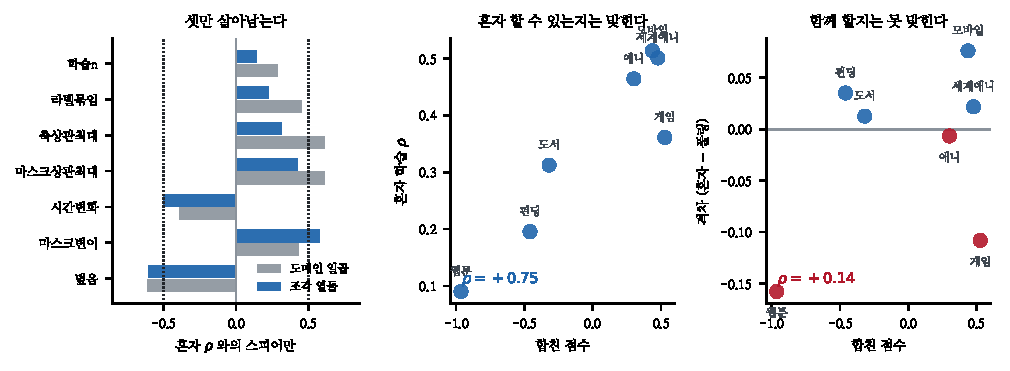
\includegraphics[width=\textwidth]{figs/alone.pdf}
\caption{왼쪽 --- 셋만 살아남는다. 가운데 --- 혼자 할 수 있는지는 맞힌다.
오른쪽 --- 함께 할지는 못 맞힌다.}
\end{figure*}

\section{후보 일곱을 걸렀다}

\begin{table}[t]
\centering\tsize
\caption{혼자 학습한 $\rho$ 와의 스피어만.}
\begin{tabular}{lrrl}
\toprule
& 도메인 7 & 조각 12 & \\
\midrule
\textbf{덮음} & \textbf{$-$.607} & \textbf{$-$.601} & 안정 \\
\textbf{마스크 변이} & $+$.429 & \textbf{$+$.573} & 안정 \\
\textbf{시간 변화} & $-$.393 & \textbf{$-$.503} & 안정 \\
\midrule
마스크상관최대 & $+$.607 & $+$.427 & 약해짐 \\
\textbf{축상관최대} & \textbf{$+$.607} & \textbf{$+$.315} & \textbf{무너짐} \\
라벨 묶임 & $+$.450 & $+$.221 & 약해짐 \\
학습 표본 & $+$.286 & $+$.140 & 부호 불안정 \\
\bottomrule
\end{tabular}
\end{table}

\claimx{\textbf{학습 표본 크기는 웹툰 하나가 만든다} --- 웹툰을 빼면 $-$0.03
에서 $+$0.77 로 뒤집힌다. 웹툰이 제일 크고(2,106행) 제일 못 배운다
($+$0.090).}{그래서 ``큰 도메인이 자립한다''는 거짓이다. 노트 197에서
풀링 이득과 학습 표본의 상관이 $-$0.07 이었던 것과 같은 방향이다.}

\claimx{\textbf{조각으로 늘리면 축상관최대가 무너진다}($+$0.607 $\to$
$+$0.315). 도메인 일곱으로는 1위였는데 조각 열둘에서는 4위다.}{조각 열둘은
독립이 아니다 --- 같은 도메인의 두 반쪽은 성질이 거의 같다. \textbf{그러니
이건 새 증거라기보다 \emph{안 흔들리는지}를 본 것이다.} 흔들린 것은 뺀다.}

\section{셋은 한 이야기다}

\begin{table}[t]
\centering\tsize
\caption{살아남은 셋. 낮은 덮음 $=$ 좋음.}
\begin{tabular}{lrrrr}
\toprule
& 혼자 $\rho$ & 덮음 & 마스크 변이 & 시간 변화 \\
\midrule
모바일 & \textbf{.514} & .635 & .076 & .123 \\
세계애니 & .501 & .681 & .053 & \textbf{.059} \\
애니 & .464 & .736 & .094 & .087 \\
게임 & .361 & \textbf{.599} & \textbf{.103} & .172 \\
도서 & .313 & .707 & .076 & .153 \\
펀딩 & .195 & .708 & .025 & .106 \\
\textbf{웹툰} & \textbf{.090} & \textbf{.749} & \textbf{.022} & .127 \\
\bottomrule
\end{tabular}
\end{table}

\claimx{\textbf{빈칸이 많고 관계가 안 변하는 도메인이 자기 자료로
배운다.} 웹툰은 덮음이 제일 높고(0.749) 마스크 변이가 제일 낮다(0.022) ---
쓸 정보가 값에만 있는데 그 값의 뜻이 시간에 변한다(노트 182).}{노트 175 ·
176 이 ``마스크는 열 수가 아니라 내용으로 값을 한다''를 세웠는데,
\textbf{여기서 그것이 도메인 수준의 성질로 나타난다.}}

\claimx{셋을 표준화해 더한 점수가 혼자 $\rho$ 를 \textbf{$+$0.750} 으로
예측한다 --- 단독 최고($+$0.607)보다 낫다.}{셋이 서로 다른 것을 재고 있다는
뜻이다. 덮음과 마스크 변이는 겹칠 것 같은데(둘 다 결측 구조) 애니가 둘 다
높아 안 겹친다.}

\section{그런데 배치는 못 정한다}

\begin{table}[t]
\centering\tsize
\caption{점수와 격차.}
\begin{tabular}{lrrr}
\toprule
& 점수 & 혼자 $\rho$ & 격차 \\
\midrule
\textbf{게임} & \textbf{0.53} & .361 & \textbf{$-$.108} \\
세계애니 & 0.48 & .501 & $+$.022 \\
\textbf{모바일} & 0.44 & \textbf{.514} & \textbf{$+$.076} \\
애니 & 0.30 & .464 & $-$.007 \\
도서 & $-$0.32 & .313 & $+$.013 \\
펀딩 & $-$0.46 & .195 & $+$.035 \\
웹툰 & $-$0.96 & .090 & $-$.158 \\
\midrule
\multicolumn{2}{l}{점수 $\leftrightarrow$ 혼자} & \multicolumn{2}{r}{\textbf{$+$.750}} \\
\multicolumn{2}{l}{점수 $\leftrightarrow$ 격차} & \multicolumn{2}{r}{\textbf{$+$.143}} \\
\bottomrule
\end{tabular}
\end{table}

\claimx{\textbf{점수 1위가 게임인데 게임은 풀링이 $+$0.108 낫다.} 빼야 하는
것은 모바일(점수 3위)이다. \textbf{점수 $\leftrightarrow$ 격차가 $+$0.143}
으로 사실상 0 이다.}{격차는 혼자에서 풀링을 뺀 것이고, 도메인 자체의 성질로는
혼자 쪽만 예측된다 --- 표준화한 (혼자 $-$ 풀링)은 격차와 $+$0.893 이지만
그건 거의 정의다.}

\claimx{\textbf{풀링 쪽은 그 도메인이 아니라 나머지 아홉이 정한다.} 게임은
혼자 $+$0.361 로 중간인데 풀링이 $+$0.469 로 크게 올라간다 --- 다른 도메인의
자료가 게임에 잘 맞기 때문이고, 그건 게임의 성질이 아니다.}{그러니 노트 202가
바란 ``새 도메인을 자료 보기 전에 배치''는 \textbf{원리적으로 반쪽만
가능하다.} 자기 학습 능력은 그 도메인만 보면 되고 풀 적합도는 판 전체를
봐야 한다.}

\begin{table}[t]
\centering\tsize
\caption{남은 것.}
\begin{tabular}{ll}
\toprule
\textbf{풀링 쪽} & 나머지 아홉과의 무엇이 풀링 적합도를 정하나 \\
셋의 무게 & 표준화해 그냥 더했다 --- 무게를 정하면 \\
조각 & 반으로 쪼갠 열둘은 독립이 아니다 \\
\bottomrule
\end{tabular}
\end{table}

첫 줄이 이 갈래에 남은 진짜 질문이다. 점수는 \emph{혼자} 항만 예측하므로,
\emph{풀링} 항을 예측하는 성질을 따로 찾아야 격차가 예측된다. 후보가 있다 ---
노트 197이 잰 도메인 쌍 계수 코사인이다. 게임은 세계애니(0.75) · 웹툰(0.71)과
계수가 제일 닮았고 그래서 풀링이 잘 맞을 수 있다. \textbf{``나머지와 얼마나
닮았나''를 점수에 더하면 격차가 예측될지 모른다} --- 노트 197에서 코사인이
풀링 \emph{이득}과 $-$0.25 로 약했는데, 그때는 혼자 항과 섞여 있었다.
\textbf{혼자 항을 따로 뺀 뒤 코사인을 대면 다르게 나올 수 있다.}

\end{document}
